\documentclass[a4paper,12pt]{article}
\usepackage{czech}
\usepackage[utf8]{inputenc}
\usepackage{a4wide}
\usepackage[dvipdfm]{graphicx}
\usepackage{graphics}
\usepackage{indentfirst}
\usepackage{fancyhdr}
\usepackage{setspace}
\usepackage{amsmath}
\usepackage{amssymb}
\usepackage{epsfig}

%%\usepackage{nopageno}
%%\usepackage{txfonts}
\usepackage[usenames]{color}


\begin{document}
\newcommand{\st}{^{\circ}}

\section{Úkol}

\begin{enumerate}
    \item Změřte současně světelnou i voltampérovou charakteristiku polovodičového laseru. Naměřené závislosti zpracujte graficky. Stanovte prahový proud $i_0$.
    \item Pomocí Hg výbojky okalibrujte stupnici monochromátoru SPM 2.
    \item Změřte emisní spektrum polovodičového laseru při několika hodnotách proudu laserem pod a nad odhadnutou prahovou hodnotou $i_0$. Určete vlnovou délku stimulované emise a kvalitativně diskutujte změny ve spektrech provázející změnu napájecího proudu.
    \item Z modové struktury emisního spektra laseru určete délku aktivní oblasti rezonátoru. Diskutujte, proč je volena velmi úzká štěrbina monochromátoru.
    \item Určete výkonovou účinnost laseru pro vybranou hodnotu proudu v nadprahové oblasti. 
\end{enumerate}

\section{Teorie}
\subsection{Laser}
Laser je světelný zdroj zpravidla úzkého spektra, který funguje na principu fotoemise. V našem případě používáme PN přechod, který se jako laser začne chovat až po překročení prakového proudu $i_0$.

\subsection{Rezonátor}
Strany přechodu laseru jsou vybroušeny tak, aby fungovala jako zrcadla. Díky tomu světlo před výstupem z laseru několikrát projde tam a zpět, přičemž vyvolává nucenou fotoemisi. Vlnění vzniklé uvnitř laseru je stojaté a proto v závislosti na délce rezonátoru musí pro vycházející světlo platit
\begin{eqnarray}
\Delta\lambda=\frac{\lambda^2}{2LN_g},
\end{eqnarray}
kde $\Delta\lambda$ je rozdíl k dalšímu maximu, $\lambda$ je vlnová délka, $L$ délka rezonátoru a $N_g$ grupová rychlost uvnitř řechodu. Pro náš laser je její hodnota
\begin{eqnarray}
N_g=4.5
\end{eqnarray}
Z tohosnadno získáme vztah pro délku
\begin{eqnarray}
L=\frac{\lambda^2}{2N_g\Delta\lambda}
\label{L}
\end{eqnarray}

\subsection{Účinnost laseru}
Účinnost laseru je definována vztahem
\begin{eqnarray}
\eta=\frac{\Phi_e}{UI},
\label{eta}
\end{eqnarray}
kde $\Phi_e$ je vyzařovaný výkon, $U$ napětí a $I$ proud.

\subsection{Chyby měření}
Veškeré chyby měření byly dány nejistotami měřidel. Použitá zařízení spolu s jejich chybami na použitém rozsahu jsou uvedeny v tabulce \ref{TCh}

\begin{table}
$$
\begin{array}{|c|c|}
\hline
\mbox{voltmetr UNI-T UT803}&  \pm (0.3 \% + 2\mbox{d}) \\ \hline
\mbox{ampérmetr RFT G-1002.500}&  \pm (0.4 \% + 3\mbox{d}) \\ \hline
\mbox{galvanometr MG5}& \mbox{třída přesnosti}\ 2 \\ \hline    
\end{array}
$$
\caption{Nejistoty měřících přístrojů.}
\label{TCh}
\end{table}

\section{Měření}
\subsection{VA charakteristika laseru}
V připraveném zapojení jsem měřil VA charakteristiku. Postupoval jsem od 
115 mA do 0 mA. Naměřené hodnoty jsou v tabulce \ref{TVA}. Zároveň jsem si zaznamenával i relativní
 světelný výkon z galvanometru, který je v tabulce uveden v počtech dílků. Výrobce udává, že při 
 proudu 115 mA je zářivý výkon laseru 0.5 mW. Z této hodnoty jsem následně vypočetl světelný výkon pro zbylé proudy uvedený ve 4. sloupci. Nakonec jsem sestavil charakteristiky, které jsou na obrázku \ref{g1}. 
\begin{table}
$$
\begin{array}{|c|c|c|c|}
\hline
U/\mbox{V}& I/\mbox{mA}& 1/\mbox{d. galva.}  &    \Phi_e/\mbox{mW} \\ \hline 
1.898\pm 0.008&  114.9\pm 0.8&  19\pm0.5& 0.50 \pm 0.01 \\ \hline
1.890\pm 0.008&  112.1\pm 0.7&  18\pm0.5& 0.47 \pm 0.01 \\ \hline
1.879\pm 0.008&  109.8\pm 0.7&  17\pm0.5& 0.45 \pm 0.01 \\ \hline
1.862\pm 0.008&  104.8\pm 0.7&  15\pm0.5& 0.39 \pm 0.01 \\ \hline
1.847\pm 0.007&  100.2\pm 0.7&  13\pm0.5& 0.34 \pm 0.01 \\ \hline
1.831\pm 0.007&  95.0\pm 0.7&   12\pm0.5& 0.32 \pm 0.01 \\ \hline
1.814\pm 0.007&  90.3\pm 0.7&   10\pm0.5& 0.26 \pm 0.01 \\ \hline
1.795\pm 0.007&  84.9\pm 0.6&   9\pm0.5&  0.24 \pm 0.01 \\ \hline
1.780\pm 0.007&  80.5\pm 0.6&   8\pm0.5&  0.21 \pm 0.01 \\ \hline
1.760\pm 0.007&  74.8\pm 0.6&   7\pm0.5&  0.18 \pm 0.01 \\ \hline
1.742\pm 0.007&  70.3\pm 0.6&   6\pm0.5&  0.16 \pm 0.01 \\ \hline
1.724\pm 0.007&  65.2\pm 0.6&   6\pm0.5&  0.16 \pm 0.01 \\ \hline
1.706\pm 0.007&  60.6\pm 0.5&   5\pm0.5&  0.13 \pm 0.01 \\ \hline
1.664\pm 0.007&  49.9\pm 0.5&   4\pm0.5&  0.11 \pm 0.01 \\ \hline
1.621\pm 0.007&  40.0\pm 0.5& 3\pm0.5&  0.08 \pm 0.01 \\ \hline
1.577\pm 0.007&  30.3\pm 0.4&2\pm0.5   &  0.05 \pm 0.01 \\ \hline
1.522\pm 0.007&  20.0\pm 0.3& 1\pm0.5&  0.03 \pm 0.01 \\ \hline
1.458\pm 0.006&  10.4\pm 0.3&1\pm 0.5   &  0.03 \pm 0.02 \\ \hline
1.403\pm 0.006&  5.0\pm 0.3&  0\pm 0.5  &  0.00 \pm 0.02 \\ \hline
1.047\pm 0.005&  0.0\pm 0.3&  0\pm 0.5 &  0.00 \pm 0.02 \\ \hline
\end{array}
$$
\caption{VA a světelná charakteristika GaAs laseru}
\label{TVA}
\end{table}

\begin{figure}
\begin{center}
% GNUPLOT: LaTeX picture with Postscript
\begingroup
  \makeatletter
  \providecommand\color[2][]{%
    \GenericError{(gnuplot) \space\space\space\@spaces}{%
      Package color not loaded in conjunction with
      terminal option `colourtext'%
    }{See the gnuplot documentation for explanation.%
    }{Either use 'blacktext' in gnuplot or load the package
      color.sty in LaTeX.}%
    \renewcommand\color[2][]{}%
  }%
  \providecommand\includegraphics[2][]{%
    \GenericError{(gnuplot) \space\space\space\@spaces}{%
      Package graphicx or graphics not loaded%
    }{See the gnuplot documentation for explanation.%
    }{The gnuplot epslatex terminal needs graphicx.sty or graphics.sty.}%
    \renewcommand\includegraphics[2][]{}%
  }%
  \providecommand\rotatebox[2]{#2}%
  \@ifundefined{ifGPcolor}{%
    \newif\ifGPcolor
    \GPcolorfalse
  }{}%
  \@ifundefined{ifGPblacktext}{%
    \newif\ifGPblacktext
    \GPblacktexttrue
  }{}%
  % define a \g@addto@macro without @ in the name:
  \let\gplgaddtomacro\g@addto@macro
  % define empty templates for all commands taking text:
  \gdef\gplbacktext{}%
  \gdef\gplfronttext{}%
  \makeatother
  \ifGPblacktext
    % no textcolor at all
    \def\colorrgb#1{}%
    \def\colorgray#1{}%
  \else
    % gray or color?
    \ifGPcolor
      \def\colorrgb#1{\color[rgb]{#1}}%
      \def\colorgray#1{\color[gray]{#1}}%
      \expandafter\def\csname LTw\endcsname{\color{white}}%
      \expandafter\def\csname LTb\endcsname{\color{black}}%
      \expandafter\def\csname LTa\endcsname{\color{black}}%
      \expandafter\def\csname LT0\endcsname{\color[rgb]{1,0,0}}%
      \expandafter\def\csname LT1\endcsname{\color[rgb]{0,1,0}}%
      \expandafter\def\csname LT2\endcsname{\color[rgb]{0,0,1}}%
      \expandafter\def\csname LT3\endcsname{\color[rgb]{1,0,1}}%
      \expandafter\def\csname LT4\endcsname{\color[rgb]{0,1,1}}%
      \expandafter\def\csname LT5\endcsname{\color[rgb]{1,1,0}}%
      \expandafter\def\csname LT6\endcsname{\color[rgb]{0,0,0}}%
      \expandafter\def\csname LT7\endcsname{\color[rgb]{1,0.3,0}}%
      \expandafter\def\csname LT8\endcsname{\color[rgb]{0.5,0.5,0.5}}%
    \else
      % gray
      \def\colorrgb#1{\color{black}}%
      \def\colorgray#1{\color[gray]{#1}}%
      \expandafter\def\csname LTw\endcsname{\color{white}}%
      \expandafter\def\csname LTb\endcsname{\color{black}}%
      \expandafter\def\csname LTa\endcsname{\color{black}}%
      \expandafter\def\csname LT0\endcsname{\color{black}}%
      \expandafter\def\csname LT1\endcsname{\color{black}}%
      \expandafter\def\csname LT2\endcsname{\color{black}}%
      \expandafter\def\csname LT3\endcsname{\color{black}}%
      \expandafter\def\csname LT4\endcsname{\color{black}}%
      \expandafter\def\csname LT5\endcsname{\color{black}}%
      \expandafter\def\csname LT6\endcsname{\color{black}}%
      \expandafter\def\csname LT7\endcsname{\color{black}}%
      \expandafter\def\csname LT8\endcsname{\color{black}}%
    \fi
  \fi
  \setlength{\unitlength}{0.0500bp}%
  \begin{picture}(7200.00,5040.00)%
    \gplgaddtomacro\gplbacktext{%
      \csname LTb\endcsname%
      \put(946,704){\makebox(0,0)[r]{\strut{} 0}}%
      \put(946,1111){\makebox(0,0)[r]{\strut{} 20}}%
      \put(946,1518){\makebox(0,0)[r]{\strut{} 40}}%
      \put(946,1925){\makebox(0,0)[r]{\strut{} 60}}%
      \put(946,2332){\makebox(0,0)[r]{\strut{} 80}}%
      \put(946,2740){\makebox(0,0)[r]{\strut{} 100}}%
      \put(946,3147){\makebox(0,0)[r]{\strut{} 120}}%
      \put(946,3554){\makebox(0,0)[r]{\strut{} 140}}%
      \put(946,3961){\makebox(0,0)[r]{\strut{} 160}}%
      \put(946,4368){\makebox(0,0)[r]{\strut{} 180}}%
      \put(946,4775){\makebox(0,0)[r]{\strut{} 200}}%
      \put(1078,484){\makebox(0,0){\strut{}-30}}%
      \put(2032,484){\makebox(0,0){\strut{}-20}}%
      \put(2986,484){\makebox(0,0){\strut{}-10}}%
      \put(3941,484){\makebox(0,0){\strut{} 0}}%
      \put(4895,484){\makebox(0,0){\strut{} 10}}%
      \put(5849,484){\makebox(0,0){\strut{} 20}}%
      \put(6803,484){\makebox(0,0){\strut{} 30}}%
      \put(176,2739){\rotatebox{-270}{\makebox(0,0){\strut{}$I$/rel. j.}}}%
      \put(3940,154){\makebox(0,0){\strut{}$x$/mm}}%
    }%
    \gplgaddtomacro\gplfronttext{%
    }%
    \gplbacktext
    \put(0,0){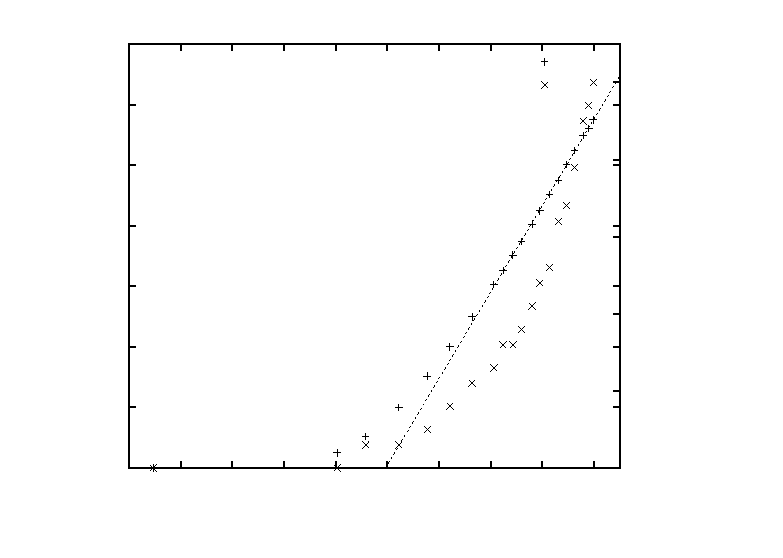
\includegraphics{g1}}%
    \gplfronttext
  \end{picture}%
\endgroup

\end{center}
\caption{VA a světelná charakteristika}
\label{g1}
\end{figure}

\subsection{Prahový proud}
Prahový proud $i_0$ by se měl pohybovat v místě kde začne proud stoupat lineárně s napětím. Dle nafitované přímky v \ref{g1} je jeho hodnota přibližně
\begin{eqnarray}
i_0=(50\pm 10) \mbox{mA}
\end{eqnarray}
Přesnější hodnotu nejsem sto určit.

\subsection{Hg výbojka}
Pomocí spektrometru počítače u úlohy jsem proměřil spektrum Hg výbojky. Z naměřených dat jsem vytvořil graf \ref{g2}. Dle tabulkových hodnot spelktrálních čar pro Hg výbojku jsem vytvožil kalibrační křivku pro spektrometr, která je na obrázku \ref{g3}. Vlnové délky odpovídající dílkům spektrometru jsou v tabulce \ref{THg}. 

\begin{table}
$$
\begin{array}{|c|c|}
\hline
\mbox{dílků s.}&   \lambda/\mbox{nm} \\ \hline
17.6109&    404.7 \\ \hline
18.2000&    435.8 \\ \hline
20.2779&    546.1 \\ \hline
\end{array}
$$
\caption{Kalibrace spektrometru}
\label{THg}
\end{table}

\begin{figure}
\begin{center}
% GNUPLOT: LaTeX picture with Postscript
\begingroup
  \makeatletter
  \providecommand\color[2][]{%
    \GenericError{(gnuplot) \space\space\space\@spaces}{%
      Package color not loaded in conjunction with
      terminal option `colourtext'%
    }{See the gnuplot documentation for explanation.%
    }{Either use 'blacktext' in gnuplot or load the package
      color.sty in LaTeX.}%
    \renewcommand\color[2][]{}%
  }%
  \providecommand\includegraphics[2][]{%
    \GenericError{(gnuplot) \space\space\space\@spaces}{%
      Package graphicx or graphics not loaded%
    }{See the gnuplot documentation for explanation.%
    }{The gnuplot epslatex terminal needs graphicx.sty or graphics.sty.}%
    \renewcommand\includegraphics[2][]{}%
  }%
  \providecommand\rotatebox[2]{#2}%
  \@ifundefined{ifGPcolor}{%
    \newif\ifGPcolor
    \GPcolorfalse
  }{}%
  \@ifundefined{ifGPblacktext}{%
    \newif\ifGPblacktext
    \GPblacktexttrue
  }{}%
  % define a \g@addto@macro without @ in the name:
  \let\gplgaddtomacro\g@addto@macro
  % define empty templates for all commands taking text:
  \gdef\gplbacktext{}%
  \gdef\gplfronttext{}%
  \makeatother
  \ifGPblacktext
    % no textcolor at all
    \def\colorrgb#1{}%
    \def\colorgray#1{}%
  \else
    % gray or color?
    \ifGPcolor
      \def\colorrgb#1{\color[rgb]{#1}}%
      \def\colorgray#1{\color[gray]{#1}}%
      \expandafter\def\csname LTw\endcsname{\color{white}}%
      \expandafter\def\csname LTb\endcsname{\color{black}}%
      \expandafter\def\csname LTa\endcsname{\color{black}}%
      \expandafter\def\csname LT0\endcsname{\color[rgb]{1,0,0}}%
      \expandafter\def\csname LT1\endcsname{\color[rgb]{0,1,0}}%
      \expandafter\def\csname LT2\endcsname{\color[rgb]{0,0,1}}%
      \expandafter\def\csname LT3\endcsname{\color[rgb]{1,0,1}}%
      \expandafter\def\csname LT4\endcsname{\color[rgb]{0,1,1}}%
      \expandafter\def\csname LT5\endcsname{\color[rgb]{1,1,0}}%
      \expandafter\def\csname LT6\endcsname{\color[rgb]{0,0,0}}%
      \expandafter\def\csname LT7\endcsname{\color[rgb]{1,0.3,0}}%
      \expandafter\def\csname LT8\endcsname{\color[rgb]{0.5,0.5,0.5}}%
    \else
      % gray
      \def\colorrgb#1{\color{black}}%
      \def\colorgray#1{\color[gray]{#1}}%
      \expandafter\def\csname LTw\endcsname{\color{white}}%
      \expandafter\def\csname LTb\endcsname{\color{black}}%
      \expandafter\def\csname LTa\endcsname{\color{black}}%
      \expandafter\def\csname LT0\endcsname{\color{black}}%
      \expandafter\def\csname LT1\endcsname{\color{black}}%
      \expandafter\def\csname LT2\endcsname{\color{black}}%
      \expandafter\def\csname LT3\endcsname{\color{black}}%
      \expandafter\def\csname LT4\endcsname{\color{black}}%
      \expandafter\def\csname LT5\endcsname{\color{black}}%
      \expandafter\def\csname LT6\endcsname{\color{black}}%
      \expandafter\def\csname LT7\endcsname{\color{black}}%
      \expandafter\def\csname LT8\endcsname{\color{black}}%
    \fi
  \fi
  \setlength{\unitlength}{0.0500bp}%
  \begin{picture}(7200.00,5040.00)%
    \gplgaddtomacro\gplbacktext{%
      \csname LTb\endcsname%
      \put(1078,704){\makebox(0,0)[r]{\strut{} 0}}%
      \put(1078,1286){\makebox(0,0)[r]{\strut{} 100}}%
      \put(1078,1867){\makebox(0,0)[r]{\strut{} 200}}%
      \put(1078,2449){\makebox(0,0)[r]{\strut{} 300}}%
      \put(1078,3030){\makebox(0,0)[r]{\strut{} 400}}%
      \put(1078,3612){\makebox(0,0)[r]{\strut{} 500}}%
      \put(1078,4193){\makebox(0,0)[r]{\strut{} 600}}%
      \put(1078,4775){\makebox(0,0)[r]{\strut{} 700}}%
      \put(1210,484){\makebox(0,0){\strut{}-8}}%
      \put(1917,484){\makebox(0,0){\strut{}-6}}%
      \put(2625,484){\makebox(0,0){\strut{}-4}}%
      \put(3332,484){\makebox(0,0){\strut{}-2}}%
      \put(4040,484){\makebox(0,0){\strut{} 0}}%
      \put(4747,484){\makebox(0,0){\strut{} 2}}%
      \put(5454,484){\makebox(0,0){\strut{} 4}}%
      \put(6162,484){\makebox(0,0){\strut{} 6}}%
      \put(6869,484){\makebox(0,0){\strut{} 8}}%
      \put(308,2739){\rotatebox{-270}{\makebox(0,0){\strut{}$H$/Am$^{-1}$}}}%
      \put(4039,154){\makebox(0,0){\strut{}$x$/cm}}%
    }%
    \gplgaddtomacro\gplfronttext{%
      \csname LTb\endcsname%
      \put(5882,4602){\makebox(0,0)[r]{\strut{}12 cm}}%
      \csname LTb\endcsname%
      \put(5882,4382){\makebox(0,0)[r]{\strut{}16 cm}}%
      \csname LTb\endcsname%
      \put(5882,4162){\makebox(0,0)[r]{\strut{}20 cm}}%
    }%
    \gplbacktext
    \put(0,0){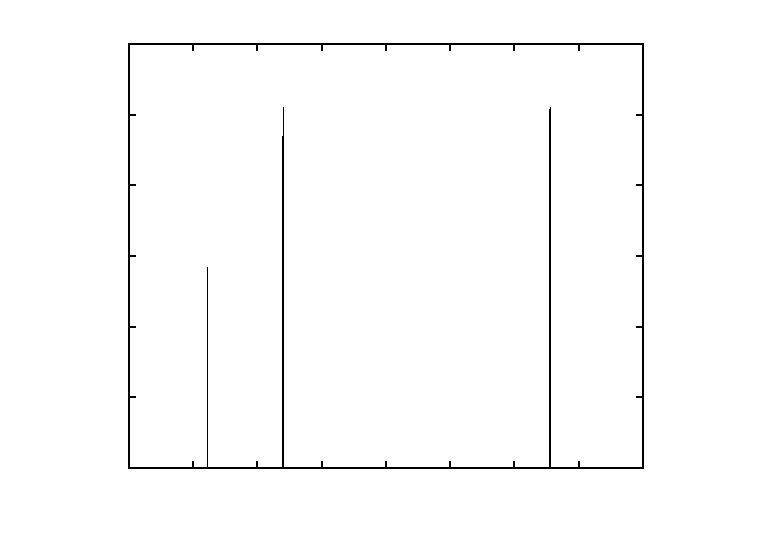
\includegraphics{g2}}%
    \gplfronttext
  \end{picture}%
\endgroup

\end{center}
\caption{Spektrum rtuťové výbojky.}
\label{g2}
\end{figure}

\begin{figure}
\begin{center}
% GNUPLOT: LaTeX picture with Postscript
\begingroup
  \makeatletter
  \providecommand\color[2][]{%
    \GenericError{(gnuplot) \space\space\space\@spaces}{%
      Package color not loaded in conjunction with
      terminal option `colourtext'%
    }{See the gnuplot documentation for explanation.%
    }{Either use 'blacktext' in gnuplot or load the package
      color.sty in LaTeX.}%
    \renewcommand\color[2][]{}%
  }%
  \providecommand\includegraphics[2][]{%
    \GenericError{(gnuplot) \space\space\space\@spaces}{%
      Package graphicx or graphics not loaded%
    }{See the gnuplot documentation for explanation.%
    }{The gnuplot epslatex terminal needs graphicx.sty or graphics.sty.}%
    \renewcommand\includegraphics[2][]{}%
  }%
  \providecommand\rotatebox[2]{#2}%
  \@ifundefined{ifGPcolor}{%
    \newif\ifGPcolor
    \GPcolorfalse
  }{}%
  \@ifundefined{ifGPblacktext}{%
    \newif\ifGPblacktext
    \GPblacktexttrue
  }{}%
  % define a \g@addto@macro without @ in the name:
  \let\gplgaddtomacro\g@addto@macro
  % define empty templates for all commands taking text:
  \gdef\gplbacktext{}%
  \gdef\gplfronttext{}%
  \makeatother
  \ifGPblacktext
    % no textcolor at all
    \def\colorrgb#1{}%
    \def\colorgray#1{}%
  \else
    % gray or color?
    \ifGPcolor
      \def\colorrgb#1{\color[rgb]{#1}}%
      \def\colorgray#1{\color[gray]{#1}}%
      \expandafter\def\csname LTw\endcsname{\color{white}}%
      \expandafter\def\csname LTb\endcsname{\color{black}}%
      \expandafter\def\csname LTa\endcsname{\color{black}}%
      \expandafter\def\csname LT0\endcsname{\color[rgb]{1,0,0}}%
      \expandafter\def\csname LT1\endcsname{\color[rgb]{0,1,0}}%
      \expandafter\def\csname LT2\endcsname{\color[rgb]{0,0,1}}%
      \expandafter\def\csname LT3\endcsname{\color[rgb]{1,0,1}}%
      \expandafter\def\csname LT4\endcsname{\color[rgb]{0,1,1}}%
      \expandafter\def\csname LT5\endcsname{\color[rgb]{1,1,0}}%
      \expandafter\def\csname LT6\endcsname{\color[rgb]{0,0,0}}%
      \expandafter\def\csname LT7\endcsname{\color[rgb]{1,0.3,0}}%
      \expandafter\def\csname LT8\endcsname{\color[rgb]{0.5,0.5,0.5}}%
    \else
      % gray
      \def\colorrgb#1{\color{black}}%
      \def\colorgray#1{\color[gray]{#1}}%
      \expandafter\def\csname LTw\endcsname{\color{white}}%
      \expandafter\def\csname LTb\endcsname{\color{black}}%
      \expandafter\def\csname LTa\endcsname{\color{black}}%
      \expandafter\def\csname LT0\endcsname{\color{black}}%
      \expandafter\def\csname LT1\endcsname{\color{black}}%
      \expandafter\def\csname LT2\endcsname{\color{black}}%
      \expandafter\def\csname LT3\endcsname{\color{black}}%
      \expandafter\def\csname LT4\endcsname{\color{black}}%
      \expandafter\def\csname LT5\endcsname{\color{black}}%
      \expandafter\def\csname LT6\endcsname{\color{black}}%
      \expandafter\def\csname LT7\endcsname{\color{black}}%
      \expandafter\def\csname LT8\endcsname{\color{black}}%
    \fi
  \fi
  \setlength{\unitlength}{0.0500bp}%
  \begin{picture}(7200.00,5040.00)%
    \gplgaddtomacro\gplbacktext{%
      \csname LTb\endcsname%
      \put(1078,704){\makebox(0,0)[r]{\strut{} 100}}%
      \put(1078,1213){\makebox(0,0)[r]{\strut{} 200}}%
      \put(1078,1722){\makebox(0,0)[r]{\strut{} 300}}%
      \put(1078,2231){\makebox(0,0)[r]{\strut{} 400}}%
      \put(1078,2740){\makebox(0,0)[r]{\strut{} 500}}%
      \put(1078,3248){\makebox(0,0)[r]{\strut{} 600}}%
      \put(1078,3757){\makebox(0,0)[r]{\strut{} 700}}%
      \put(1078,4266){\makebox(0,0)[r]{\strut{} 800}}%
      \put(1078,4775){\makebox(0,0)[r]{\strut{} 900}}%
      \put(1210,484){\makebox(0,0){\strut{} 0}}%
      \put(2153,484){\makebox(0,0){\strut{} 5}}%
      \put(3096,484){\makebox(0,0){\strut{} 10}}%
      \put(4039,484){\makebox(0,0){\strut{} 15}}%
      \put(4983,484){\makebox(0,0){\strut{} 20}}%
      \put(5926,484){\makebox(0,0){\strut{} 25}}%
      \put(6869,484){\makebox(0,0){\strut{} 30}}%
      \put(308,2739){\rotatebox{-270}{\makebox(0,0){\strut{}$R/\Omega$}}}%
      \put(4039,154){\makebox(0,0){\strut{}$I/$mA}}%
    }%
    \gplgaddtomacro\gplfronttext{%
      \csname LTb\endcsname%
      \put(4774,4602){\makebox(0,0)[r]{\strut{}substituční metoda}}%
      \csname LTb\endcsname%
      \put(4774,4382){\makebox(0,0)[r]{\strut{}přímá metoda s korekcí}}%
    }%
    \gplbacktext
    \put(0,0){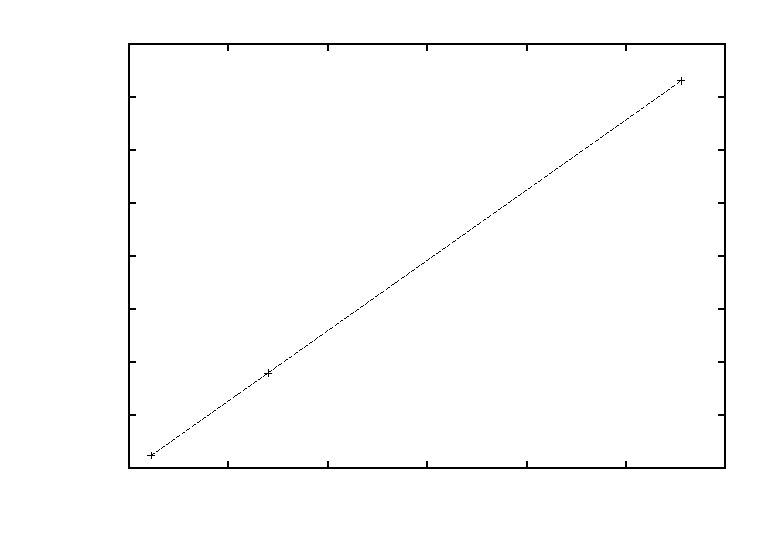
\includegraphics{g3}}%
    \gplfronttext
  \end{picture}%
\endgroup

\end{center}
\caption{Kalibrační křivk pro spektrometr.}
\label{g3}
\end{figure}

Vzrah pro vlnovou délku vypočítanou z dílků spektrometru je
\begin{eqnarray}
\lambda=(53.04\pm 0.05)*x-(529.36\pm 1.00) \mbox{nm}
\end{eqnarray}


\subsection{Spektrum laseru}
Za pomoci naměřených hodnot a kalibrační křivky \ref{g3} jsem vytvořil graf spektra GaAs laseru pro různé hodnoty proudu. Výsledek je na obrázku \ref{g4}. Zněj jsem určil vlnovou délku stimulované emise, která odpovídá maximu v grafu
\begin{eqnarray}
\lambda_{max}=(812.4 \pm 0.2) \mbox{nm}
\end{eqnarray}

\begin{figure}
\begin{center}
% GNUPLOT: LaTeX picture with Postscript
\begingroup
  \makeatletter
  \providecommand\color[2][]{%
    \GenericError{(gnuplot) \space\space\space\@spaces}{%
      Package color not loaded in conjunction with
      terminal option `colourtext'%
    }{See the gnuplot documentation for explanation.%
    }{Either use 'blacktext' in gnuplot or load the package
      color.sty in LaTeX.}%
    \renewcommand\color[2][]{}%
  }%
  \providecommand\includegraphics[2][]{%
    \GenericError{(gnuplot) \space\space\space\@spaces}{%
      Package graphicx or graphics not loaded%
    }{See the gnuplot documentation for explanation.%
    }{The gnuplot epslatex terminal needs graphicx.sty or graphics.sty.}%
    \renewcommand\includegraphics[2][]{}%
  }%
  \providecommand\rotatebox[2]{#2}%
  \@ifundefined{ifGPcolor}{%
    \newif\ifGPcolor
    \GPcolorfalse
  }{}%
  \@ifundefined{ifGPblacktext}{%
    \newif\ifGPblacktext
    \GPblacktexttrue
  }{}%
  % define a \g@addto@macro without @ in the name:
  \let\gplgaddtomacro\g@addto@macro
  % define empty templates for all commands taking text:
  \gdef\gplbacktext{}%
  \gdef\gplfronttext{}%
  \makeatother
  \ifGPblacktext
    % no textcolor at all
    \def\colorrgb#1{}%
    \def\colorgray#1{}%
  \else
    % gray or color?
    \ifGPcolor
      \def\colorrgb#1{\color[rgb]{#1}}%
      \def\colorgray#1{\color[gray]{#1}}%
      \expandafter\def\csname LTw\endcsname{\color{white}}%
      \expandafter\def\csname LTb\endcsname{\color{black}}%
      \expandafter\def\csname LTa\endcsname{\color{black}}%
      \expandafter\def\csname LT0\endcsname{\color[rgb]{1,0,0}}%
      \expandafter\def\csname LT1\endcsname{\color[rgb]{0,1,0}}%
      \expandafter\def\csname LT2\endcsname{\color[rgb]{0,0,1}}%
      \expandafter\def\csname LT3\endcsname{\color[rgb]{1,0,1}}%
      \expandafter\def\csname LT4\endcsname{\color[rgb]{0,1,1}}%
      \expandafter\def\csname LT5\endcsname{\color[rgb]{1,1,0}}%
      \expandafter\def\csname LT6\endcsname{\color[rgb]{0,0,0}}%
      \expandafter\def\csname LT7\endcsname{\color[rgb]{1,0.3,0}}%
      \expandafter\def\csname LT8\endcsname{\color[rgb]{0.5,0.5,0.5}}%
    \else
      % gray
      \def\colorrgb#1{\color{black}}%
      \def\colorgray#1{\color[gray]{#1}}%
      \expandafter\def\csname LTw\endcsname{\color{white}}%
      \expandafter\def\csname LTb\endcsname{\color{black}}%
      \expandafter\def\csname LTa\endcsname{\color{black}}%
      \expandafter\def\csname LT0\endcsname{\color{black}}%
      \expandafter\def\csname LT1\endcsname{\color{black}}%
      \expandafter\def\csname LT2\endcsname{\color{black}}%
      \expandafter\def\csname LT3\endcsname{\color{black}}%
      \expandafter\def\csname LT4\endcsname{\color{black}}%
      \expandafter\def\csname LT5\endcsname{\color{black}}%
      \expandafter\def\csname LT6\endcsname{\color{black}}%
      \expandafter\def\csname LT7\endcsname{\color{black}}%
      \expandafter\def\csname LT8\endcsname{\color{black}}%
    \fi
  \fi
  \setlength{\unitlength}{0.0500bp}%
  \begin{picture}(7200.00,5040.00)%
    \gplgaddtomacro\gplbacktext{%
      \csname LTb\endcsname%
      \put(946,1010){\makebox(0,0)[r]{\strut{} 20}}%
      \put(946,1481){\makebox(0,0)[r]{\strut{} 40}}%
      \put(946,1951){\makebox(0,0)[r]{\strut{} 60}}%
      \put(946,2422){\makebox(0,0)[r]{\strut{} 80}}%
      \put(946,2892){\makebox(0,0)[r]{\strut{} 100}}%
      \put(946,3363){\makebox(0,0)[r]{\strut{} 120}}%
      \put(946,3834){\makebox(0,0)[r]{\strut{} 140}}%
      \put(946,4304){\makebox(0,0)[r]{\strut{} 160}}%
      \put(946,4775){\makebox(0,0)[r]{\strut{} 180}}%
      \put(1078,484){\makebox(0,0){\strut{} 790}}%
      \put(2032,484){\makebox(0,0){\strut{} 800}}%
      \put(2986,484){\makebox(0,0){\strut{} 810}}%
      \put(3941,484){\makebox(0,0){\strut{} 820}}%
      \put(4895,484){\makebox(0,0){\strut{} 830}}%
      \put(5849,484){\makebox(0,0){\strut{} 840}}%
      \put(6803,484){\makebox(0,0){\strut{} 850}}%
      \put(176,2739){\rotatebox{-270}{\makebox(0,0){\strut{}rel. intenzita}}}%
      \put(3940,154){\makebox(0,0){\strut{}$\lambda$/nm}}%
    }%
    \gplgaddtomacro\gplfronttext{%
      \csname LTb\endcsname%
      \put(5816,4602){\makebox(0,0)[r]{\strut{}80.0 mA}}%
      \csname LTb\endcsname%
      \put(5816,4382){\makebox(0,0)[r]{\strut{}90.1 mA}}%
      \csname LTb\endcsname%
      \put(5816,4162){\makebox(0,0)[r]{\strut{}100.2 mA}}%
      \csname LTb\endcsname%
      \put(5816,3942){\makebox(0,0)[r]{\strut{}110.1 mA}}%
      \csname LTb\endcsname%
      \put(5816,3722){\makebox(0,0)[r]{\strut{}114.3 mA}}%
    }%
    \gplbacktext
    \put(0,0){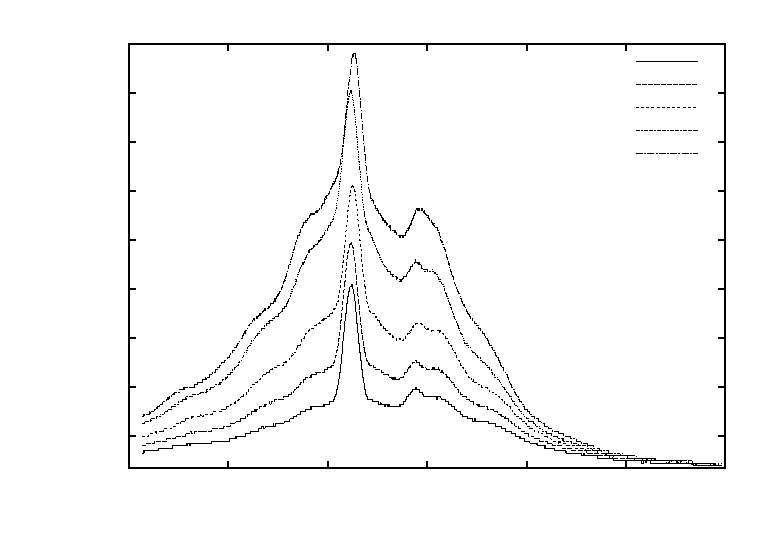
\includegraphics{g4}}%
    \gplfronttext
  \end{picture}%
\endgroup

\end{center}
\caption{Spektrum GaAs laseru pro různé hodnoty proudu.}
\label{g4}
\end{figure}

\begin{figure}
\begin{center}
% GNUPLOT: LaTeX picture with Postscript
\begingroup
  \makeatletter
  \providecommand\color[2][]{%
    \GenericError{(gnuplot) \space\space\space\@spaces}{%
      Package color not loaded in conjunction with
      terminal option `colourtext'%
    }{See the gnuplot documentation for explanation.%
    }{Either use 'blacktext' in gnuplot or load the package
      color.sty in LaTeX.}%
    \renewcommand\color[2][]{}%
  }%
  \providecommand\includegraphics[2][]{%
    \GenericError{(gnuplot) \space\space\space\@spaces}{%
      Package graphicx or graphics not loaded%
    }{See the gnuplot documentation for explanation.%
    }{The gnuplot epslatex terminal needs graphicx.sty or graphics.sty.}%
    \renewcommand\includegraphics[2][]{}%
  }%
  \providecommand\rotatebox[2]{#2}%
  \@ifundefined{ifGPcolor}{%
    \newif\ifGPcolor
    \GPcolorfalse
  }{}%
  \@ifundefined{ifGPblacktext}{%
    \newif\ifGPblacktext
    \GPblacktexttrue
  }{}%
  % define a \g@addto@macro without @ in the name:
  \let\gplgaddtomacro\g@addto@macro
  % define empty templates for all commands taking text:
  \gdef\gplbacktext{}%
  \gdef\gplfronttext{}%
  \makeatother
  \ifGPblacktext
    % no textcolor at all
    \def\colorrgb#1{}%
    \def\colorgray#1{}%
  \else
    % gray or color?
    \ifGPcolor
      \def\colorrgb#1{\color[rgb]{#1}}%
      \def\colorgray#1{\color[gray]{#1}}%
      \expandafter\def\csname LTw\endcsname{\color{white}}%
      \expandafter\def\csname LTb\endcsname{\color{black}}%
      \expandafter\def\csname LTa\endcsname{\color{black}}%
      \expandafter\def\csname LT0\endcsname{\color[rgb]{1,0,0}}%
      \expandafter\def\csname LT1\endcsname{\color[rgb]{0,1,0}}%
      \expandafter\def\csname LT2\endcsname{\color[rgb]{0,0,1}}%
      \expandafter\def\csname LT3\endcsname{\color[rgb]{1,0,1}}%
      \expandafter\def\csname LT4\endcsname{\color[rgb]{0,1,1}}%
      \expandafter\def\csname LT5\endcsname{\color[rgb]{1,1,0}}%
      \expandafter\def\csname LT6\endcsname{\color[rgb]{0,0,0}}%
      \expandafter\def\csname LT7\endcsname{\color[rgb]{1,0.3,0}}%
      \expandafter\def\csname LT8\endcsname{\color[rgb]{0.5,0.5,0.5}}%
    \else
      % gray
      \def\colorrgb#1{\color{black}}%
      \def\colorgray#1{\color[gray]{#1}}%
      \expandafter\def\csname LTw\endcsname{\color{white}}%
      \expandafter\def\csname LTb\endcsname{\color{black}}%
      \expandafter\def\csname LTa\endcsname{\color{black}}%
      \expandafter\def\csname LT0\endcsname{\color{black}}%
      \expandafter\def\csname LT1\endcsname{\color{black}}%
      \expandafter\def\csname LT2\endcsname{\color{black}}%
      \expandafter\def\csname LT3\endcsname{\color{black}}%
      \expandafter\def\csname LT4\endcsname{\color{black}}%
      \expandafter\def\csname LT5\endcsname{\color{black}}%
      \expandafter\def\csname LT6\endcsname{\color{black}}%
      \expandafter\def\csname LT7\endcsname{\color{black}}%
      \expandafter\def\csname LT8\endcsname{\color{black}}%
    \fi
  \fi
  \setlength{\unitlength}{0.0500bp}%
  \begin{picture}(7200.00,5040.00)%
    \gplgaddtomacro\gplbacktext{%
      \csname LTb\endcsname%
      \put(946,704){\makebox(0,0)[r]{\strut{} 40}}%
      \put(946,1213){\makebox(0,0)[r]{\strut{} 60}}%
      \put(946,1722){\makebox(0,0)[r]{\strut{} 80}}%
      \put(946,2231){\makebox(0,0)[r]{\strut{} 100}}%
      \put(946,2740){\makebox(0,0)[r]{\strut{} 120}}%
      \put(946,3248){\makebox(0,0)[r]{\strut{} 140}}%
      \put(946,3757){\makebox(0,0)[r]{\strut{} 160}}%
      \put(946,4266){\makebox(0,0)[r]{\strut{} 180}}%
      \put(946,4775){\makebox(0,0)[r]{\strut{} 200}}%
      \put(1078,484){\makebox(0,0){\strut{} 795}}%
      \put(1714,484){\makebox(0,0){\strut{} 800}}%
      \put(2350,484){\makebox(0,0){\strut{} 805}}%
      \put(2986,484){\makebox(0,0){\strut{} 810}}%
      \put(3622,484){\makebox(0,0){\strut{} 815}}%
      \put(4259,484){\makebox(0,0){\strut{} 820}}%
      \put(4895,484){\makebox(0,0){\strut{} 825}}%
      \put(5531,484){\makebox(0,0){\strut{} 830}}%
      \put(6167,484){\makebox(0,0){\strut{} 835}}%
      \put(6803,484){\makebox(0,0){\strut{} 840}}%
      \put(176,2739){\rotatebox{-270}{\makebox(0,0){\strut{}relativní intenzita}}}%
      \put(3940,154){\makebox(0,0){\strut{}$\lambda$/nm}}%
    }%
    \gplgaddtomacro\gplfronttext{%
      \csname LTb\endcsname%
      \put(5816,4602){\makebox(0,0)[r]{\strut{}první měřnení}}%
      \csname LTb\endcsname%
      \put(5816,4382){\makebox(0,0)[r]{\strut{}druhé měření}}%
    }%
    \gplbacktext
    \put(0,0){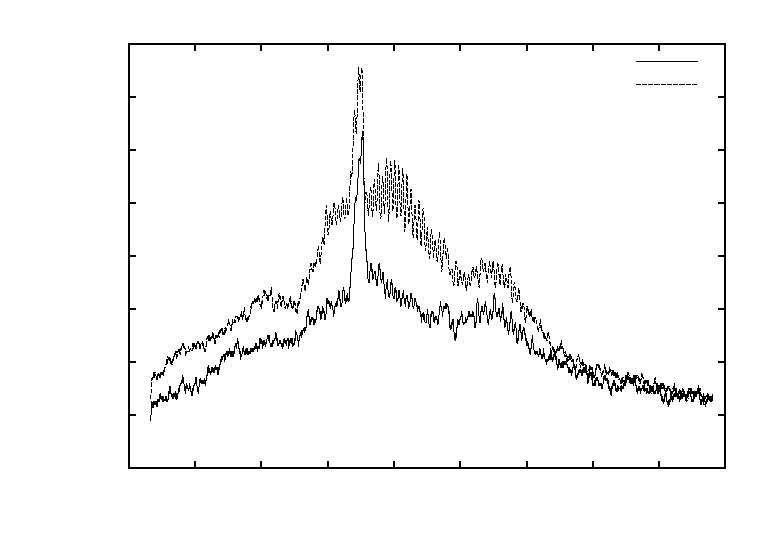
\includegraphics{g5}}%
    \gplfronttext
  \end{picture}%
\endgroup

\end{center}
\caption{Emisní spektrum GaAs laseru při úzké štěrbině.}
\label{g5}
\end{figure}

\begin{figure}
\begin{center}
% GNUPLOT: LaTeX picture with Postscript
\begingroup
  \makeatletter
  \providecommand\color[2][]{%
    \GenericError{(gnuplot) \space\space\space\@spaces}{%
      Package color not loaded in conjunction with
      terminal option `colourtext'%
    }{See the gnuplot documentation for explanation.%
    }{Either use 'blacktext' in gnuplot or load the package
      color.sty in LaTeX.}%
    \renewcommand\color[2][]{}%
  }%
  \providecommand\includegraphics[2][]{%
    \GenericError{(gnuplot) \space\space\space\@spaces}{%
      Package graphicx or graphics not loaded%
    }{See the gnuplot documentation for explanation.%
    }{The gnuplot epslatex terminal needs graphicx.sty or graphics.sty.}%
    \renewcommand\includegraphics[2][]{}%
  }%
  \providecommand\rotatebox[2]{#2}%
  \@ifundefined{ifGPcolor}{%
    \newif\ifGPcolor
    \GPcolorfalse
  }{}%
  \@ifundefined{ifGPblacktext}{%
    \newif\ifGPblacktext
    \GPblacktexttrue
  }{}%
  % define a \g@addto@macro without @ in the name:
  \let\gplgaddtomacro\g@addto@macro
  % define empty templates for all commands taking text:
  \gdef\gplbacktext{}%
  \gdef\gplfronttext{}%
  \makeatother
  \ifGPblacktext
    % no textcolor at all
    \def\colorrgb#1{}%
    \def\colorgray#1{}%
  \else
    % gray or color?
    \ifGPcolor
      \def\colorrgb#1{\color[rgb]{#1}}%
      \def\colorgray#1{\color[gray]{#1}}%
      \expandafter\def\csname LTw\endcsname{\color{white}}%
      \expandafter\def\csname LTb\endcsname{\color{black}}%
      \expandafter\def\csname LTa\endcsname{\color{black}}%
      \expandafter\def\csname LT0\endcsname{\color[rgb]{1,0,0}}%
      \expandafter\def\csname LT1\endcsname{\color[rgb]{0,1,0}}%
      \expandafter\def\csname LT2\endcsname{\color[rgb]{0,0,1}}%
      \expandafter\def\csname LT3\endcsname{\color[rgb]{1,0,1}}%
      \expandafter\def\csname LT4\endcsname{\color[rgb]{0,1,1}}%
      \expandafter\def\csname LT5\endcsname{\color[rgb]{1,1,0}}%
      \expandafter\def\csname LT6\endcsname{\color[rgb]{0,0,0}}%
      \expandafter\def\csname LT7\endcsname{\color[rgb]{1,0.3,0}}%
      \expandafter\def\csname LT8\endcsname{\color[rgb]{0.5,0.5,0.5}}%
    \else
      % gray
      \def\colorrgb#1{\color{black}}%
      \def\colorgray#1{\color[gray]{#1}}%
      \expandafter\def\csname LTw\endcsname{\color{white}}%
      \expandafter\def\csname LTb\endcsname{\color{black}}%
      \expandafter\def\csname LTa\endcsname{\color{black}}%
      \expandafter\def\csname LT0\endcsname{\color{black}}%
      \expandafter\def\csname LT1\endcsname{\color{black}}%
      \expandafter\def\csname LT2\endcsname{\color{black}}%
      \expandafter\def\csname LT3\endcsname{\color{black}}%
      \expandafter\def\csname LT4\endcsname{\color{black}}%
      \expandafter\def\csname LT5\endcsname{\color{black}}%
      \expandafter\def\csname LT6\endcsname{\color{black}}%
      \expandafter\def\csname LT7\endcsname{\color{black}}%
      \expandafter\def\csname LT8\endcsname{\color{black}}%
    \fi
  \fi
  \setlength{\unitlength}{0.0500bp}%
  \begin{picture}(7200.00,5040.00)%
    \gplgaddtomacro\gplbacktext{%
      \csname LTb\endcsname%
      \put(946,704){\makebox(0,0)[r]{\strut{} 100}}%
      \put(946,1111){\makebox(0,0)[r]{\strut{} 110}}%
      \put(946,1518){\makebox(0,0)[r]{\strut{} 120}}%
      \put(946,1925){\makebox(0,0)[r]{\strut{} 130}}%
      \put(946,2332){\makebox(0,0)[r]{\strut{} 140}}%
      \put(946,2740){\makebox(0,0)[r]{\strut{} 150}}%
      \put(946,3147){\makebox(0,0)[r]{\strut{} 160}}%
      \put(946,3554){\makebox(0,0)[r]{\strut{} 170}}%
      \put(946,3961){\makebox(0,0)[r]{\strut{} 180}}%
      \put(946,4368){\makebox(0,0)[r]{\strut{} 190}}%
      \put(946,4775){\makebox(0,0)[r]{\strut{} 200}}%
      \put(1078,484){\makebox(0,0){\strut{} 810}}%
      \put(1896,484){\makebox(0,0){\strut{} 812}}%
      \put(2714,484){\makebox(0,0){\strut{} 814}}%
      \put(3532,484){\makebox(0,0){\strut{} 816}}%
      \put(4349,484){\makebox(0,0){\strut{} 818}}%
      \put(5167,484){\makebox(0,0){\strut{} 820}}%
      \put(5985,484){\makebox(0,0){\strut{} 822}}%
      \put(6803,484){\makebox(0,0){\strut{} 824}}%
      \put(176,2739){\rotatebox{-270}{\makebox(0,0){\strut{}relativní intenzita}}}%
      \put(3940,154){\makebox(0,0){\strut{}$\lambda$/nm}}%
    }%
    \gplgaddtomacro\gplfronttext{%
    }%
    \gplbacktext
    \put(0,0){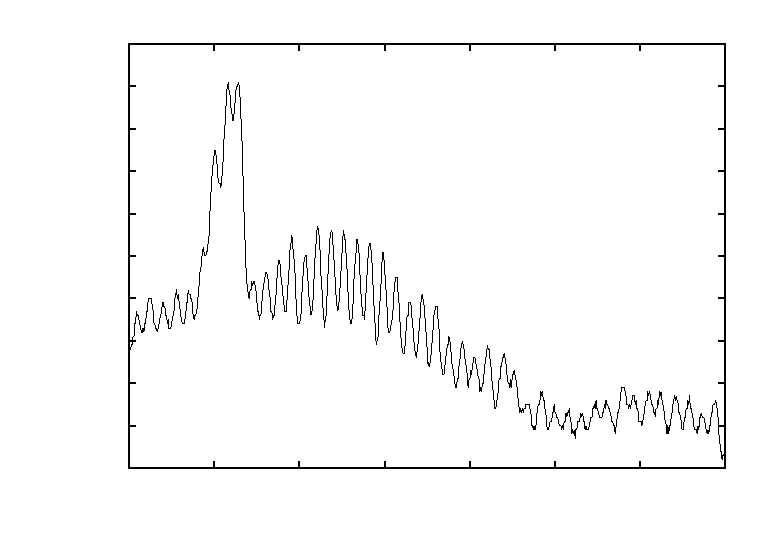
\includegraphics{g6}}%
    \gplfronttext
  \end{picture}%
\endgroup

\end{center}
\caption{Emisní spektrum GaAs laseru při úzké štěrbině.}
\label{g6}
\end{figure}


\subsection{Rezonátor}
Při nastavení velkého proudu laserem (118.5 mA) a úzké štěrbině jsem naměřil spektrum laseru s viditelnou módovou strukturou. Výsledky jsou v grafu \ref{g5}. Při prvním měření byl laser příliš daleko od spektrometru. Z druhého měření jsem vybral užšší část spektra (obrázek \ref{g6}) a z té dle vztahu \ref{L} dopočítal délku rezonátoru.
\begin{eqnarray}
l=(235.8 \pm 0.8) \mu\mbox{m}
\end{eqnarray}

\subsection{účinnost}
Po dosazení do vzorce \ref{eta} jsem stanovil účinnost laseru pro proud 114.9 mA. Výseldek je
\begin{eqnarray}
\eta = 0.23\ \%
\end{eqnarray}

\section{Diskuze}
Při měření charakteristik nedošlo k žádnému odkolu od teorie. U světelné jsou všah hodnoty podle mého názoru nižší než uvedené výše. Relativní poměr odpovídá skutečnosti, referenční hodnota pro prou 115 mA platí pro nový laser, což ten při měření použitý není.

Kalibrace spektrometru vyšla velmi dobře. V datech z měření spektra Hg výbojky jsou sice viditelné pouze tři nejvýraznější spektrální čáry (což podle mě neodpovídá grafu zobrazenému na počítači u úlohy), avšak jim nafitovaná přímka má velmi malou chybu fitu.

Spektrum laseru má dle očekávání poměrně ostré maximum. Je sice o něco výše než oblast kalibrace, ale to podle méh názoru nemá velký vliv na přesnost měření. Při zvyšování proudu rostla intenzita v celé šíři měřeného spektra. Nejvýrazněji však právě ve zmíněném maximu, které odpovídá hodnotě stimulované emise.

Při měřenímodové struktury emisního spektra jsem musel kvůli nevýraznosti prvního provést měření druhé, ve kterém je již mnohem lépe vidět potřebný jev. Pro srovnání uvádím měření obě. Úzká štěrbina byla zvolena, protože rozdíl mezi maximy je natolik malý, že při šířce vstupní štěrbyni by se jinak rozmazala. Vypočítaná hodnota délky rezonátoru by mohla odpovídat skutečnosti, ale nemám žádnou možnost porovnání správnosti výsledku.

Účinnost laseru vyšla menší, než jsem očekával. Zářivý výkon byl, jak již bylo uvedeno výše, podle mě ještě nižší, takže skutečný výkon je pravděpodobně ještě nižší.



\section{Závěr}
Naměřil jsem VA a světelnou charakteristiku GaAs laseru. Výsledek je na obrázku \ref{g1}. \\
Odhadl jsem hodnotu nprahového proudu na
\begin{eqnarray}
i_0=(50\pm 10)\mbox{mA}
\end{eqnarray}
Provedl jsem kalibraci spektrometr za pomoci Hg výbojky. Kalibrační křivka je na obrázku \ref{g3}. \\
Proměřil jsem spektrum GaAs laseru pro různé proudy. Výsledek je na obrázku \ref{g4}. \\
Určil jsem délku akrivní oblasti laseru
\begin{eqnarray}
l=(235.8 \pm 0.8)\mu\mbox{m}
\end{eqnarray}
Určil jsem výkonovou účinost laseru pro proud 114.9 mA
\begin{eqnarray}
\eta = 0.23\ \%
\end{eqnarray}

\begin{thebibliography}{5}
	\bibitem{text} \textbf{Studijní text na praktikum III} \\http://physics.mff.cuni.cz/vyuka/zfp/txt\_315.htm (28. 2. 2012)
    \bibitem{chyba} \emph{J. Englich}: \textbf{Zpracování výsldků fyzikálních měření} \\ LS 1999/2000
\end{thebibliography}


\end{document}
